\chapter{Istniejące rozwiązania}

W niniejszym rozdziale przedstawiono wybrane z istniejących rozwiązań wykorzystywanych w obszarze sportów zespołowych. Dla poszczególnych platform zostały wyszczególnione ich główne założenia oraz funkcjonalności wpływające na usprawnienie komunikacji pomiędzy sportowcami.


\section{Playarena.pl}

Rozwiązaniem, które w najbliższy sposób realizuje cele zdefiniowane we wstępnie tej pracy jest polski portal Playarena. Playarena.pl jest specjalistycznym portalem skierowanym do drużyn piłki nożnej 6-osobowej. Celem jego twórców jest zachęcanie ludzi do gry, dostarczanie możliwości rywalizacji, rozwoju oraz zabawy \cite{playarena}.

Po rejestracji w systemie użytkownicy mogą zakładać swoje drużyny lub dołączać do istniejących poprzez system aplikacji oraz zaproszeń. Głównym obszarem działania portalu są mecze ligowe, w których uczestniczyć mogą skompletowane drużyny. Kapitanowie drużyn mają możliwość rzucania wyzwań innym drużynom w swojej lidze. Najlepsze drużyny awansują do wyższych lig, a zawodnicy wypatrzeni przez łowców talentów mogą otrzymać powołanie do Reprezentacji Polski w piłce nożnej 6-osobowej. Przykładową tabelę ligową przedstawiono na rysunku \ref{fig:ss-playarena}.

Rozgrywki odbywają się na obiektach sportowych, które są zgłaszane oraz weryfikowane przez użytkowników systemu.

\begin{figure}[H]
\centering
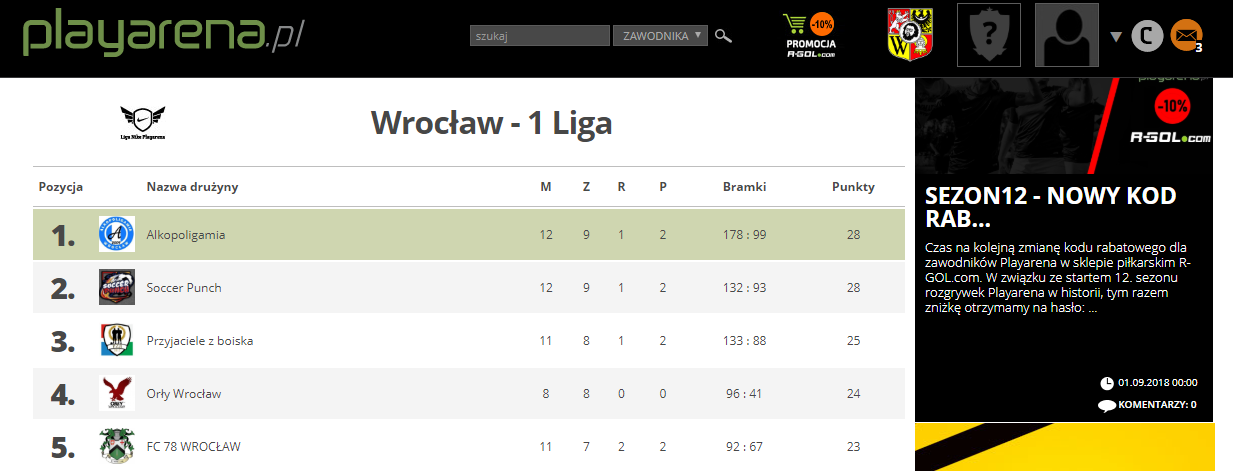
\includegraphics[width=\linewidth]{02-istniejace-rozwiazania/rys/playarena.PNG}
\caption{Przykładowy widok serwisu Playarena.pl}
\label{fig:ss-playarena}
\end{figure}


\section{SportsManago}

Na polskim rynku istnieją również rozwiązania wspomagające komunikację w obrębie amatorskich klubów sportowych oraz zarządzanie nimi. Jednym z takich rozwiązań jest \textit{SportsManago}, czyli wielofunkcyjne narzędzie usprawniające przepływ informacji między menedżerami, trenerami, zawodnikami oraz ich rodzicami. Pomysłodawcą i wykonawcą projektu jest Witold Dyjur - Absolwent Wydziału Elektroniki Politechniki Wrocławskiej.

Narzędzie umożliwia gromadzenie informacji o klubie, kartotek jego zawodników, historii meczy wraz ze szczegółowymi statystykami. \textit{SportsManago} wspiera między innymi: 

\begin{itemize}
    \item sprawdzanie obecności na treningach,
    \item prowadzenie naborów do klubu,
    \item zarządzanie obozami,
    \item zarządzanie zawodami.
\end{itemize}

Dużym usprawnieniem jest zastosowany system powiadomień SMS (ang. \textit{Short Message Service}), który pozwala na szybkie dostarczanie informacji na temat treningów, meczy i innych wydarzeń.

% \begin{figure}[H]
% \centering
% 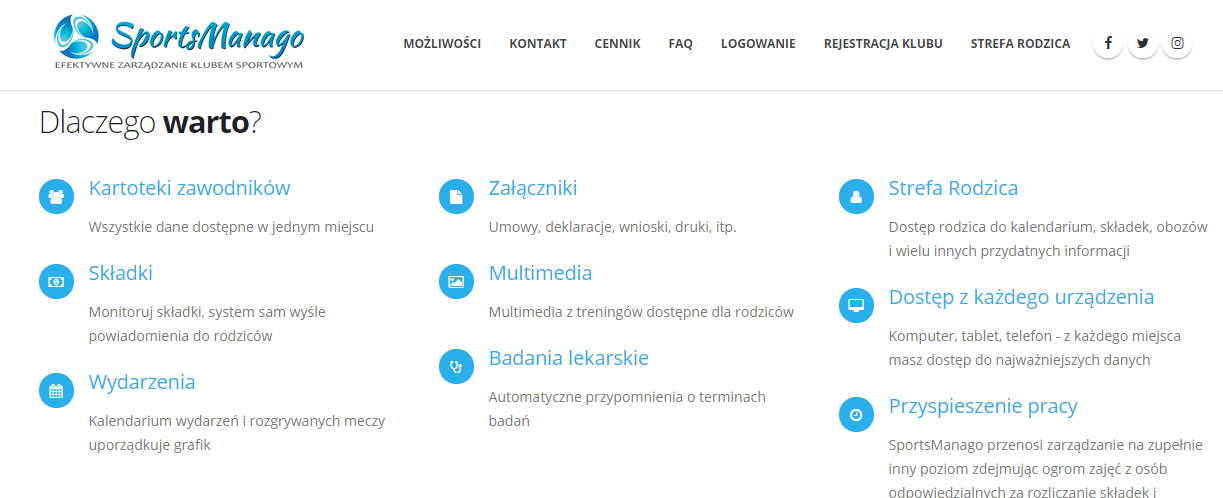
\includegraphics[width=\linewidth]{02-istniejace-rozwiazania/rys/ss-manago.PNG}
% \caption{Przykładowe funkcjonalności serwisu SportsManago}
% \label{fig:ss-manago}
% \end{figure}



\section{SportsMatchMaker.com.au}

Przykładem zagranicznego rozwiązania jest \textit{SportsMatchMaker}, czyli Australijska sieć służąca do komunikacji pomiędzy sportowcami \cite{smmau}. 

Działanie systemu przypomina tablicę ogłoszeń. Użytkownicy mogą deklarować się jako poszukujący osób do wspólnego uprawniania sportów. Ogłoszenie zawiera takie informacje jak: dyscyplina sportu, poziom zaawansowania oraz lokalizacja. Przeglądanie ofert polega na wyszukiwaniu z możliwością zawężenia wyników do określonej dyscypliny oraz lokalizacji. Przykładowe wyniki wyszukiwania osób grających w koszykówkę zostały przedstawione na rysunku \ref{fig:ss-austr}. Nawiązanie kontaktu odbywa się za pomocą wiadomości prywatnych.


\begin{figure}[H]
\centering
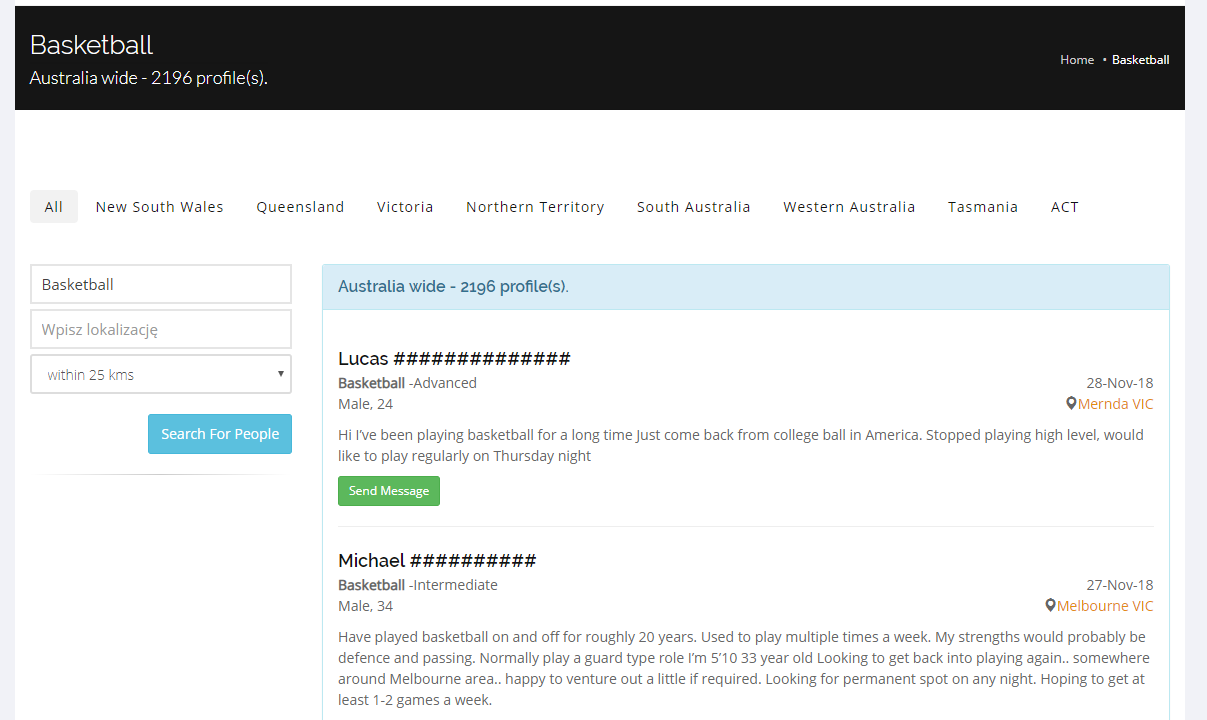
\includegraphics[width=\linewidth]{02-istniejace-rozwiazania/rys/ss-austr.PNG}
\caption{Przykładowy widok systemu SportsMatchMaker.com.au}
\label{fig:ss-austr}
\end{figure}



\section{Facebook}

Poza specjalistycznymi systemami, których głównym celem jest wspieranie sportowców, istnieją również platformy, których głównych założenia mogą wydawać się odległe. \textit{Facebook} jest serwisem społecznościowym zrzeszającym prawie 2 miliardy osób z całego świata. Główną misją \textit{Facebook-a} jest zbliżanie do siebie ludzi poprzez umożliwianie budowy społeczności \cite{fb}.

Społeczność osób uprawiających sporty zespołowe nie stanowi tutaj wyjątku. Na \textit{Facebook-u} istnieje bardzo dużo grup tematycznych, których celem jest gromadzenie osób uprawiających pewną dyscyplinę sportu w określonym regionie. Osoby organizujące rozgrywki bardzo często tworzą posty podając takie informacje jak miejsce oraz termin spotkania, preferowany wiek oraz poziom umiejętności. Chętne osoby zgłaszają się pod postem lub poprzez wiadomość prywatną. Przykładowy post został przedstawiony na rysunku \ref{fig:ss-fb}.

\begin{figure}[H]
\centering

\includegraphics[width=0.6\linewidth]{02-istniejace-rozwiazania/rys/ss-fb.PNG}
\caption{Przykładowy post użytkownika szukającego towarzyszy do gry na portalu~Facebook}
\label{fig:ss-fb}
\end{figure}


Szukanie osób do gry poprzez portal \textit{Facebook} jest bardzo często wybieranym rozwiązaniem głownie ze względu na dużą ilość użytkowników oraz szeroką dostępność serwisu. W tabeli \ref{tab:fbgrupy} przedstawiono zestawienie wybranych z publicznych grup w mieście Wrocław.


\begin{table}[htb]
\centering\small
\caption{Przykładowe grupy dla zawodników na Facebook - stan z dnia 20.11.2018r}
\label{tab:fbgrupy}
\begin{tabularx}{\linewidth}{|p{.55\linewidth}|X|}\hline
Nazwa grupy & Liczba członków \\ \hline\hline
Piłka nożna Wrocław & 4689  \\ \hline
Siatkówka Wrocław & 4460  \\ \hline
Koszykówka Wrocław & 1686 \\ \hline
Piłka nożna Wrocław - dla PWR & 273  \\ \hline
\end{tabularx}
\end{table}
